\chapter{Experiments}
\label{sec:experiments}

%%%%%%%%%%%%%%%%%%%%% Kurze Einführung %%%%%%%%%%%%%%%%%%%%%

This chapter describes all experiments conducted in this work to either develop a functional rail track prediction system or improve existing methods.
The structure can be roughly divided into the following categories:

\begin{enumerate}
    \item For an initial approach to combine object detection with semantic segmentation, experiments with object detectors are conducted and described in \autoref{sec:objectDetectionExperiments}.
    \item TEP-Net \cite{tepNet2024} is chosen as the new baseline for further improvements in accuracy and robustness. Experiments include an adapted cropping mechanism for inference (\autoref{sec:autocropExperiments}) and various changes in the model architecture (\autoref{sec:improvedTEPNETExperiments}).
    \item An additional approach to enhancing robustness involves integrating temporal information, thereby addressing the limitation of single-frame-based methods. Experiments are depicted in \autoref{sec:temporalModelsExperiments}.
\end{enumerate}

%%%%%%%%%%%%%%%%%%%%%%%%%% Object Detection Experiments %%%%%%%%%%%%%%%%%%%%%%%%%%

\section{Object detection Experiments}

The first approach pursued in this work is to combine an object detection model and a semantic segmentation model.
The semantic segmentation model should predict the track on a pixel level, and the object detection model predicts the direction of the train in scenarios where switches divide the track.

Experiments started with training object detection models from the \ac{YOLO} series.
The models \ac{YOLO}v7 \cite{yolov7} and \ac{YOLO}v9 \cite{YOLOv9} are selected to investigate their ability to predict switches and their states.
Experiments have been conducted with RailSem19 and subsets of this dataset, which are further described in \autoref{sec:usedDatasetsYOLOs}.
At the time \ac{YOLO}v9 has just been released.
Consequently, not all models were fully supported during the experiments.
Therefore, the versions \ac{GELAN}-c and \ac{GELAN}-e are utilized.
For the \ac{YOLO}v7 the smallest version with the highest reported speed is used.
Many experiments are conducted with these three models, however only the best-performing are described.

All \ac{YOLO} models have built-in data augmentation.
This includes a horizontal flip of images.
Since this horizontal flip of images only flips images but does not change the label $switch\_left$ to $switch\_right$ and vice versa, this strategy cannot be used.
Consequently, the probability of such flips is defined to be zero. The remaining default data augmentation is utilized in all experiments.
Additionally, all other default hyperparameters are not changed, and parameters that are specified in the training command are used as they are recommended in the GitHub repositories \cite{YOLOv7GitHub} and \cite{YOLOv9GitHub}.
All changed and specified parameters of the best-performing experiments are shown in \autoref{tab:usedParametersYOLOs}.
Furthermore, all models come with pre-trained weights trained on the COCO dataset.
In all experiments, these weights are used as initialization.

\begin{table}[H]
    \centering
    \begin{tabular}{|l|c|c|}
    %\begin{tabular}{| p{0.3\linewidth} | p{0.6\linewidth} |}
        \hline
        \textbf{Parameters} & \textbf{YOLOv9 models} & \textbf{YOLOv7}\\
        \hline
        img\_size & $640 \times 640$ & $640 \times 640$ \\
        \hline
        epochs & $500$ & $500$\\
        \hline
        fliplr & $0.0$ & $0.0$\\
        \hline
        batch\_size& $16$ & $16$\\
        \hline
        workers & $8$ & $8$\\
        \hline
        min-items & $0$ & \\
        \hline
        close-mosaic & $15$ & \\
        \hline
    \end{tabular}
    \caption{Used parameters for training \ac{YOLO} object detection models}
    \label{tab:usedParametersYOLOs}
\end{table}

%%%%%%%%%%%%%%%%%%%%%%%%%% Improved Autocropper %%%%%%%%%%%%%%%%%%%%%%%%%%

\section{Autocrop Experiments}
\label{sec:autocropExperiments}

Since only image crops are used in the training of all regression models, the model must get similar inputs in inference.
Therefore, an autocrop technique is introduced in \cite{tepNet2024}, and an improved version is proposed in this work in \autoref{sec:imporvedAutocrop}.
The introduced version of this mechanism includes an \ac{EMA} instead of the \ac{RA} and a proposed reset rule.
The final version stems from the results of many experiments, which are described in this section.

First, behaviors from the original cropping method proposed by \cite{tepNet2024} are analyzed.
After that, the improved version is implemented with an \ac{EMA}.
The next version includes a reset rule.
Observations show that all models result in similar behaviors when uncertain.
The horizon line of the prediction converges to the bottom of the image.
This behavior is used for the reset rule, which resets the image crop to pre-defined crop coordinates.
This is done when the prediction falls below a threshold calculated with a pre-defined percentage of the crop height.
Experiments with other versions of this reset rule are conducted.
On the one hand, various percentages are tested, and on the other hand, different reset crop coordinates are used.
Thresholds include 30\%, 40\%, 50\%, and 60\% of the crop height and crop coordinates include the whole image like \autoref{func:resetRuleParams1} and smaller crops like \autoref{func:resetRuleParams2} or \autoref{func:resetRuleParams3}, with $H=image\_height$ and $W=image\_width$.
These experiments have been conducted on real and difficult video footage in a scenario that resembles a practical application and a scenario in which the reset is forced every five seconds to test its capabilities intensively.

\begin{align}
    (left=0, top=1, right=1)
    \label{func:resetRuleParams1}
\end{align}
\begin{align}
    (left=\frac{1}{4}*W, top=\frac{1}{3}*H, right=\frac{3}{4}*W)
    \label{func:resetRuleParams2}
\end{align}
\begin{align}
    (left=\frac{1}{3}*W, top=\frac{1}{2}*H, right=\frac{2}{3}*W)
    \label{func:resetRuleParams3}
\end{align}


\noindent Further experiments are conducted with versions that stay in a fixed aspect ratio.
This ratio depends on the crop-top parameter.
First, the middle is found between the left and right coordinates.
From this middle line, the distances are calculated considering the aspect ratio and the top parameter of the crop.
Then, the left and right coordinates are overwritten.
Two aspect ratios are tested.
On the one hand, a ratio of 16:9 because images of the dataset also have this aspect ratio with a resolution of 1920 $\times$ 1080.
On the other hand, a 1:1 or a quadratic one is utilized.
Both experiments also include the \ac{EMA} and the rest rule with $(\frac{1}{3}, \frac{1}{2}, \frac{2}{3})$ because it showed the best results and the most advantageous behavior.

An additional experiment is conducted, in which the initial crop starts with the whole image width but only 10\% of the image height.
This should allow the model to find the right rail faster and build the correct crop from the bottom instead of slowly converging from the whole image to a smaller crop.
For this experiment also the \ac{EMA} and the reset rule with $(\frac{1}{3}, \frac{1}{2}, \frac{2}{3})$ is used.

All of these different versions of the auto crop mechanism are evaluated either on videos through behavioral analysis or on the switch evaluation dataset.



%%%%%%%%%%%%%%%%%%%%%%%%%% Improved TEP-Net %%%%%%%%%%%%%%%%%%%%%%%%%%

\section{Improved TEP-Net}
\label{sec:improvedTEPNETExperiments}

Various adaptations improve the performance of the model.
Experiments always consider one aspect of the architecture.
Then, the best model is used to improve performance further.
First experiments utilize different backbones.
After evaluating models' performances with various backbone versions, one is selected based on the best combination of accuracy and speed for further experiments.
The next stage applies pooling layers.
The best-performing model is then equipped with different prediction heads, resulting in models of which one again outperforms its competitors.
This model defines the final model architecture.

All trainings of different architectures utilize the same hyperparameters to compare resulting models fairly.
Numerous parameters from \cite{tepNet2024} are utilized as a basis for the guideline.
All experiments, which include adaptations of the baseline model, are pre-trained on COCO and fine-tuned on the RailSem19 dataset with the annotations of \cite{tepNet2024}.
Images of this dataset are randomly assigned to one of three subdatasets for training, validation, and testing with proportions of $80\%-10\%-10\%$.
For reproducibility of experiments, a seed of 42 is given.
Since models are solely trained on image crops, the size of these crops is set to $3 \times 512 \times 512$, which is nearest to crops from practical use cases.
Furthermore, the Adam optimizer \cite{pytorchAdamOptimizer}, in combination with the OneCycle scheduler \cite{pytorch_oneCycleLR_docu} from PyTorch, is used for training models.
First, the scheduler increases the learning rate to 0.0001 and then reduces it.
Models are all trained with a batch size of 8 for 400 epochs.

Additionally, the settings for data augmentation stay the same for all experiments with various models.
The image variation settings include factors for brightness, contrast, and saturation of 0.5.
The hue factor is set to 0.2.
These values are inspired by \cite{tepNet2024}.
However, changes in this work have been done for cropping parameters.
The margins to the top and the sides are increased to 0.2.
The standard deviation factors for the sides and the top are set to 0.3 and 0.1, respectively.

\subsection{Backbones}

In this work, experiments with four different backbones are conducted.
\cite{tepNet2024} has experimented with various ResNet and EfficientNets versions.
Literature shows that MobileNets and DenseNets have also introduced significant advancements.
The expected results of tests with DenseNets are high accuracies.
When training models that incorporate MobileNets, an advantage in latency speed is expected.
Therefore, all versions of those two network architectures are implemented that are available in PyTorch \cite{pytorchmobilenetv3} \cite{pytorchdensenet}.
\autoref{tab:backboneVersions} overviews all backbones and their versions utilized in this work.
Additionally, \autoref{subsubsec:backbones} explains the used layers.
Since all backbones must be interchangeable, this work discards some backbone layers.

\subsection{Pooling Layers}

This work either uses an adaptive average pool or an adaptive max pool to transform the output tensor of the backbone.
After reducing this tensor to a defined channel size with a \textit{conv2D1x1} layer, the pooling layers are responsible for additionally encoding spatial features into a vector-like tensor with dimensions of $C \times 1 \times 1$.
\autoref{subsubsec:pooling} gives a detailed description of the pooling layer's implementation.

\subsection{Prediction Heads}

Furthermore, experiments include various prediction heads.
This work implements a depth-head, a width-head, and a trapeze-head.
These parts of the architecture differ in the number of \ac{FC} layers and the size of these layers.
All of them result in an output vector with a pre-defined size.
A size of 129 ($2 \times H + 1$ with $H = 64$) was predominantly utilized.

\vspace{0.5cm}

\noindent Additional experiments include an input size of $3 \times 224 \times 224$, batch normalization before each ReLu activation function, and various numbers of anchors like 257 ($2 \times H + 1$ with $H = 128$).
A performance gain is strived for in each experiment.
The smaller image size is recommended in all papers of the backbones and larger numbers of anchors should give more detailed outputs.
 
%The reduced image size is chosen because all four papers of the backbones recommend this size.
%The increased number of anchors should give a more detailed description of the predicted rail track.

%%%%%%%%%%%%%%%%%%%%%%%%%% Temporal Models %%%%%%%%%%%%%%%%%%%%%%%%%%

\section{Temporal Models}
\label{sec:temporalModelsExperiments}

Training temporal models requires changes in the data-handling logic of the training processes and a new temporal dataset.
Models are trained with videos instead of single images.
Therefore, this work creates a novel sequential dataset consisting of 38 sequences with 76 frames each in which trains drive over switches.
It includes polyline labels for the left and right rail, like the dataset used to train all single-frame-based models.
\autoref{sec:tempDataset} describes this dataset in more detail.

The sequential approach in this work resembles a sequence-to-one problem.
The input consists of a predefined number of images, and the model predicts the rails in the last image.
Therefore, this work follows a sliding window method, which iterates through sequences.

In most cases, the single-frame-based model achieves high accuracy except when the train is located directly on the switch and the switchblades are not visible.
Therefore, all temporal experiments use feature extractors that are pre-trained on the single-frame dataset.
Additionally, since these backbones already extract the most relevant features, their weights are frozen, so they do not change in training.

To find the best-performing network architecture and training strategy, a large amount of experiments and evaluations are conducted in this work.
These include different data augmentation strategies, various model architectures trained on different versions of the temporal dataset, and multiple evaluation techniques.

\subsection{Data Augmentation}

Augmenting temporal data is similar to augmenting single-frame data.
However, they must be adjusted to augment a set of images instead of creating new augmentations for each video frame.
The data augmentation strategy is described in \autoref{sec:dataAugmentationTemporal} in more detail.
It incorporates color variations, random horizontal flips, and random crops.
These three techniques are utilized in various combinations, using all three, only flips and crops, solely the random crops, or no augmentation at all.
Data augmentation randomizes each window and not the whole sequence because it operates in an online fashion.
The window that iterates through a sequence includes ten images in most experiments and is smaller than the sequence length of 76.
The combination of online data augmentation and an iterating window presents an issue, especially for color variations and random flips, since different variations can appear in one sequence.
Results show that restricting data augmentation to random crops is the most advantageous method.
Leading to a new version of the sequential dataset.
The whole dataset is flipped and attached at the back to compensate for the loss in data augmentation and variety in data.
This way, the model trains without random flips within a sequence but still shows enhancements in accuracy because more data is available.

\subsection{Temporal Dataset}

Furthermore, while experimenting with temporal models, a key factor of the dataset is observed.
The dataset also includes switch cases where one of the two possible paths continues in a straight line, and the other one splits off.
The train often drives on the straight one.
In these cases, single-frame-based models usually predict the rail track correctly, as visualized in \autoref{fig:temporalTestSet_a}.
The dataset is reviewed to evaluate performances in various situations, resulting in one deleted sequence and a changed arrangement.
The new version of the dataset consists of 37 sequences, of which four are still used for validation and four for testing.
In both subsets, the single-frame model predicted each frame of these sequences with one sequence being completely wrong, one entirely correct, and two partly correct.
These sequences are selected to represent possible situations.


\begin{figure}[H]
    \centering
    \begin{subfigure}[b]{0.48\textwidth}
        \centering
        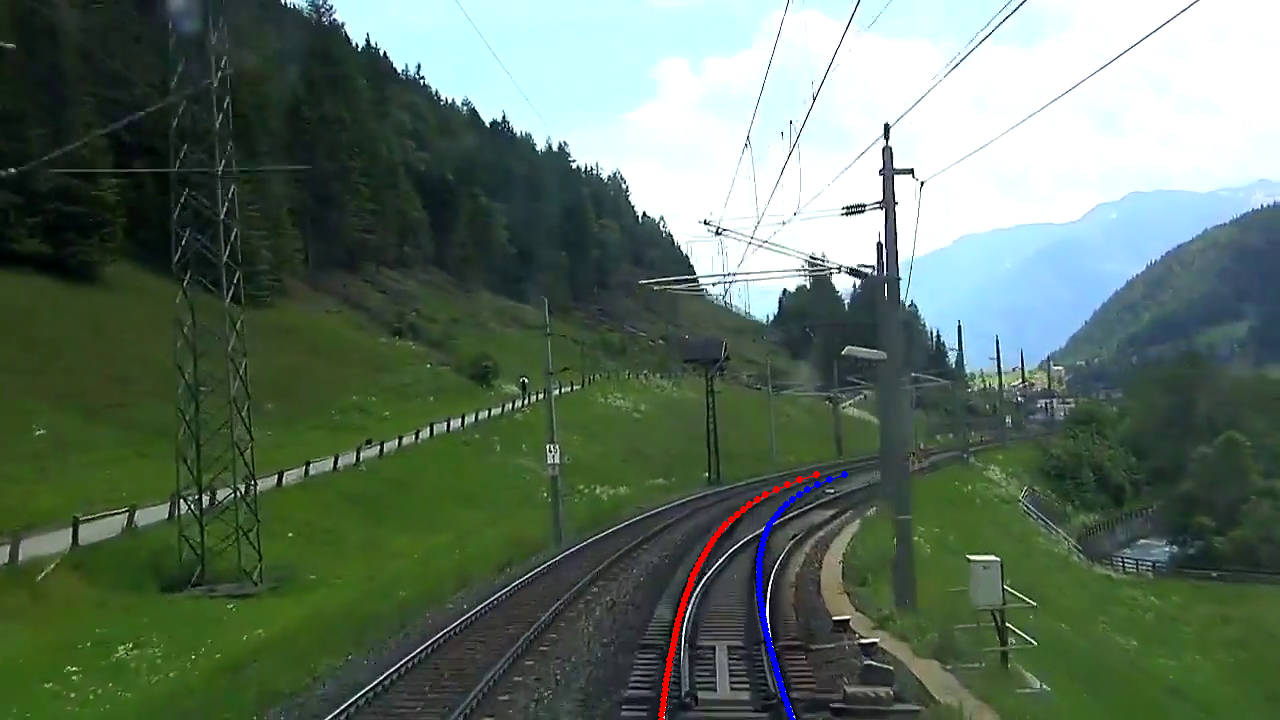
\includegraphics[width=\textwidth]{PICs/experiments/temporalModels/allesRichtig.png}
        \caption{\textbf{Switch 1}: 76/76 frames correct}
        \label{fig:temporalTestSet_a}
    \end{subfigure}
    \hfill
    \begin{subfigure}[b]{0.48\textwidth}
        \centering
        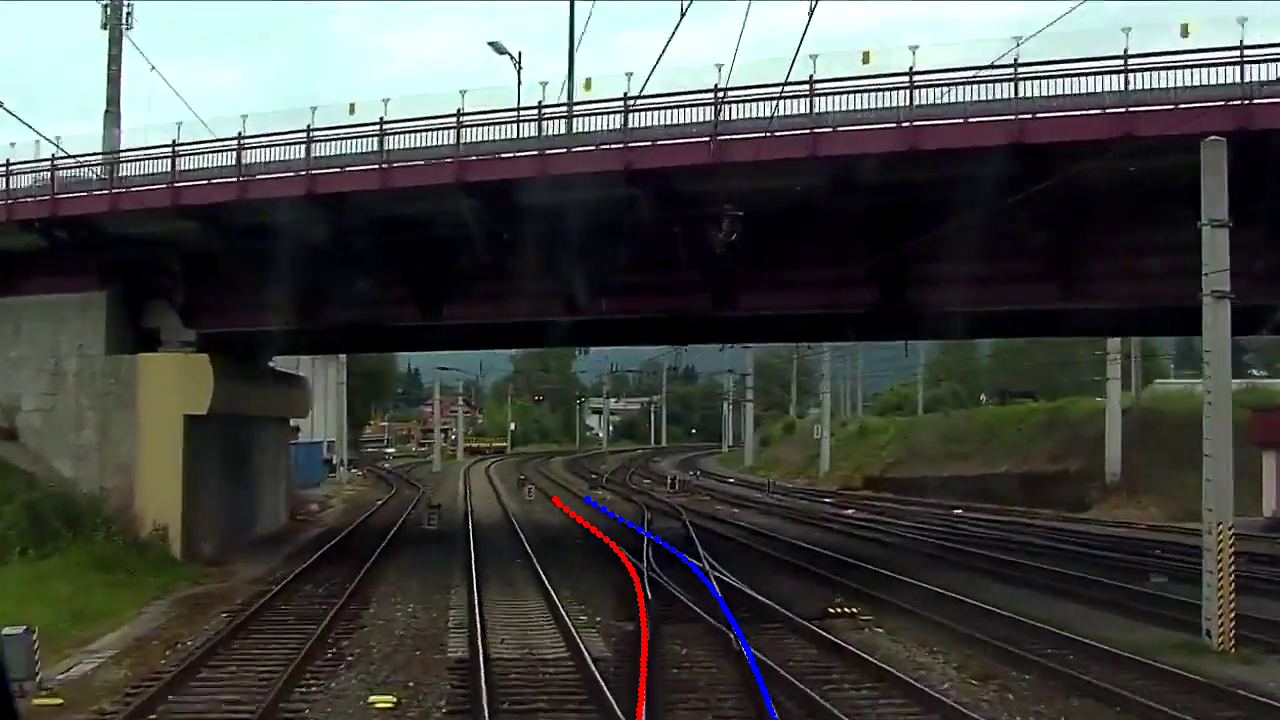
\includegraphics[width=\textwidth]{PICs/experiments/temporalModels/allesFalsch.png}
        \caption{\textbf{Switch 2}: 0/76 frames correct}
    \end{subfigure}
    
    \vspace{0.5cm} % Abstand zwischen den Zeilen

    \begin{subfigure}[b]{0.48\textwidth}
        \centering
        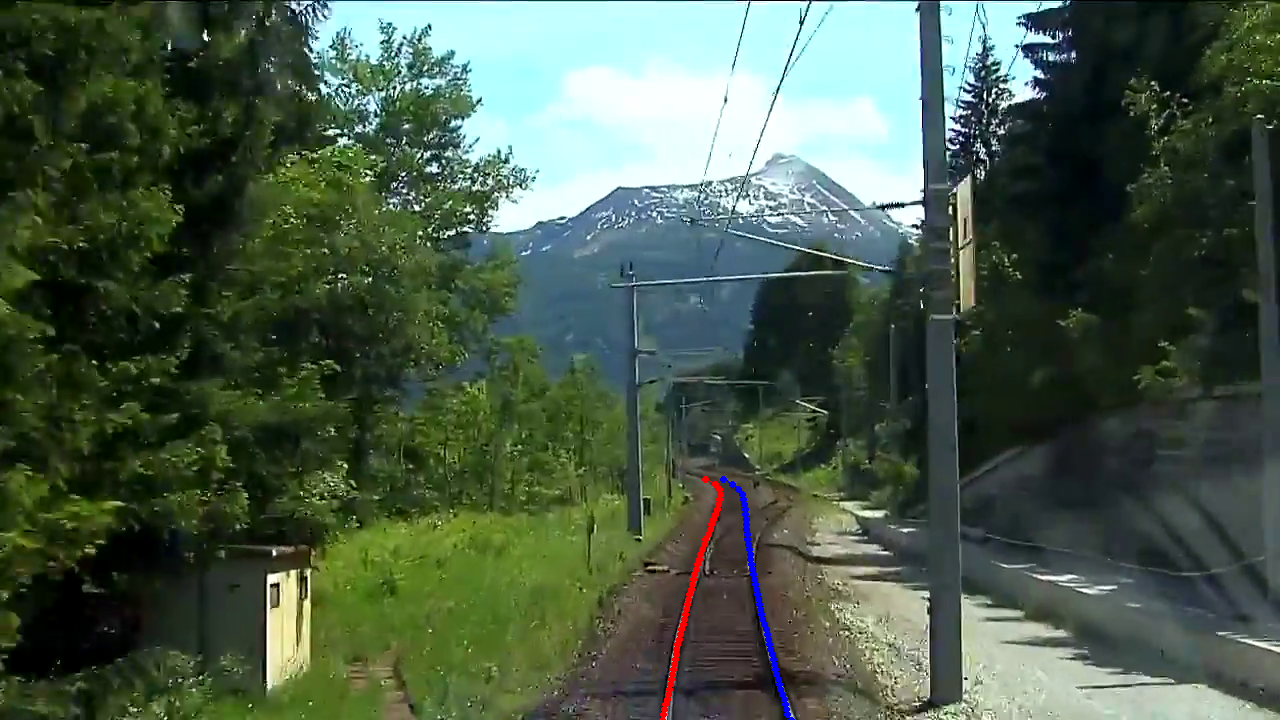
\includegraphics[width=\textwidth]{PICs/experiments/temporalModels/partlyRichtig.png}
        \caption{\textbf{Switch 3}: 36/76 frames correct}
    \end{subfigure}
    \hfill
    \begin{subfigure}[b]{0.48\textwidth}
        \centering
        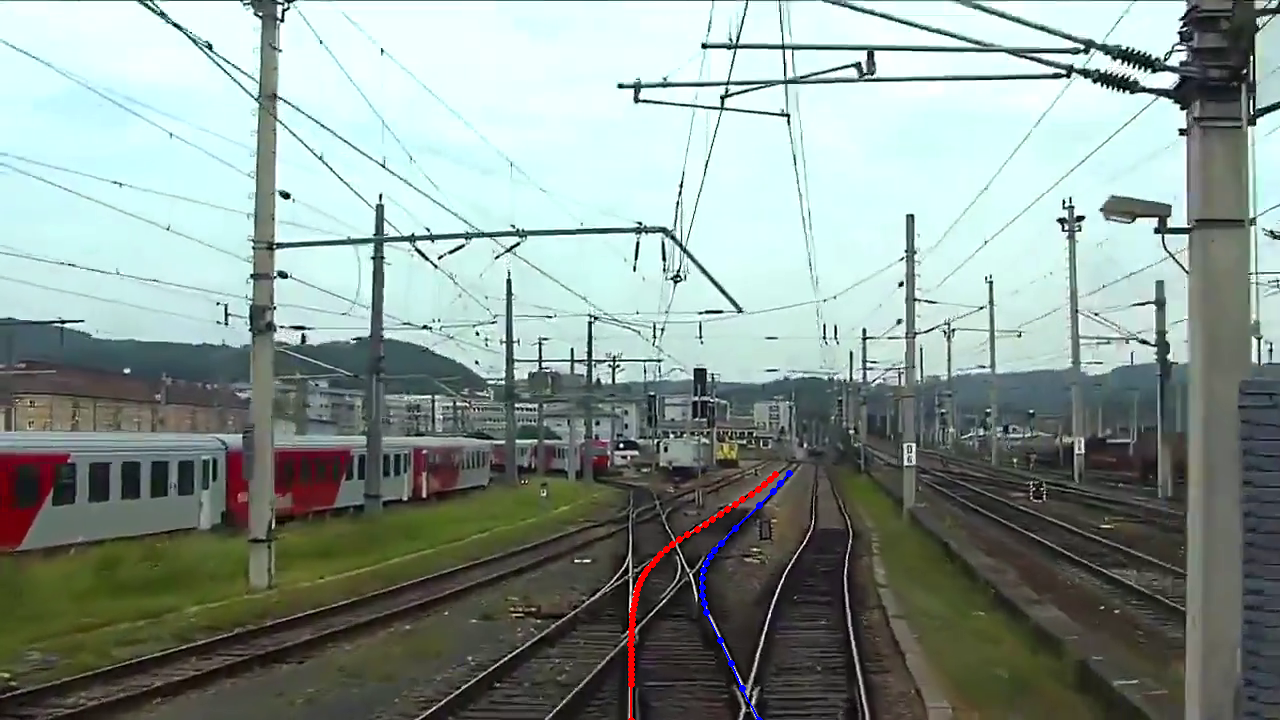
\includegraphics[width=\textwidth]{PICs/experiments/temporalModels/partlyRichtig2.png}
        \caption{\textbf{Switch 4}: 39/76 frames correct}
    \end{subfigure}
    \caption{Temporal test set with annotation. Visualized are the first images of a sequence. The number of correctly predicted frames from the single-frame-based model is in the description.}
    \label{fig:temporalTestSet}
\end{figure}

\subsection{Hyperparameters}

Most experiments, especially the latest ones, are done with the same hyperparameters to provide a fair comparison.
The best-performing single-frame-based model inspires the values used.
That is why the input dimensions are set to $3 \times 512 \times 512$.
Features are extracted with the EfficientNet-B3 backbone in all temporal experiments.
All values for data augmentation, such as color factors, crop margins, or standard deviation factors, are the same.
Furthermore, sequential experiments utilize the Adam optimizer \cite{pytorchAdamOptimizer} and a OneCycle Scheduler \cite{pytorch_oneCycleLR_docu} with the same learning rate parameters.
The best results of single-frame models are obtained with 64 anchors in the output vector.
Therefore, temporal experiments use the same number of anchors.
However, some parameters are altered.
The added complexity of sequential models significantly increases training durations.
Therefore, models train for only 100 epochs in most experiments.
Additionally, the data-handling logic within and before the model sometimes requires a batch size of 1.
Consequently, all different sequential models train with that batch size.
Furthermore, this work adds two hyperparameters to manage sequences and the sliding window.
The sequence length of 76 can be defined if the dataset changes, and the window length can be set.
Most experiments use a window length of 10 frames.
\autoref{tab:temporalExperimetparams} describes the most relevant experiments and includes the parameters used.

\begin{table}[H]
    \centering
    \resizebox{\textwidth}{!}{
    \begin{tabular}{lcccccccccc}
        \hline
        \rowcolor{white} \textbf{Model} & \multicolumn{2}{c}{\textbf{Pre-trained}} & \multicolumn{2}{c}{\textbf{Freezed}} & \multicolumn{3}{c}{\textbf{Data augmentation}} & \textbf{Sliding window} & \textbf{Epochs} & \textbf{Dataset} \\
        \hline
        \rowcolor[gray]{0.9} architecture                & BB & Head (anchors) & BB & Head   & color & flip & crop & length & number & version \\ 
        \hline
        \rowcolor{white}     CNN\_LSTM\_FC               & ENB3 & trapeze (64) & \checkmark &            & \checkmark & \checkmark & \checkmark & 10 & 107 & 1 \\ 
        \rowcolor[gray]{0.9} CNN\_FC\_LSTM               & ENB3 & trapeze (32) & \checkmark & \checkmark & \checkmark & \checkmark & \checkmark & 10 & 400 & 1 \\ 
        \rowcolor{white}     CNN\_LSTM\_V1               & ENB3 &              & \checkmark &            & \checkmark & \checkmark & \checkmark & 10 & 400 & 1 \\
        \rowcolor[gray]{0.9} CNN\_FC\_FCOUT\_V1          & ENB3 & trapeze (64) & \checkmark & \checkmark & \checkmark & \checkmark & \checkmark & 10 & 600 & 1 \\
        \hline
        \rowcolor{white}     CNN\_FC\_LSTM               & ENB3 & trapeze (32) & \checkmark & \checkmark &            & \checkmark & \checkmark & 10 & 400 & 1 \\
        \rowcolor{white}     CNN\_FC\_LSTM               & ENB3 & trapeze (32) & \checkmark & \checkmark &            &            & \checkmark & 10 & 400 & 1 \\
        \rowcolor{white}     CNN\_FC\_LSTM               & ENB3 & trapeze (32) & \checkmark & \checkmark &            &            &            & 10 & 400 & 1 \\
        \rowcolor[gray]{0.9} CNN\_LSTM\_V1               & ENB3 &              & \checkmark &            &            & \checkmark & \checkmark & 10 & 400 & 1 \\
        \rowcolor[gray]{0.9} CNN\_LSTM\_V1               & ENB3 &              & \checkmark &            &            &            & \checkmark & 10 & 400 & 1 \\
        \rowcolor[gray]{0.9} CNN\_LSTM\_V1               & ENB3 &              & \checkmark &            &            &            &            & 10 & 400 & 1 \\
        \rowcolor[gray]{0.9} CNN\_FC\_FCOUT\_V1          & ENB3 & trapeze (64) & \checkmark & \checkmark &            & \checkmark & \checkmark & 10 & 600 & 1 \\
        \rowcolor{white}     CNN\_FC\_FCOUT\_V1          & ENB3 & trapeze (64) & \checkmark & \checkmark &            &            & \checkmark & 10 & 600 & 1 \\
        \hline
        \rowcolor[gray]{0.9} CNN\_FC\_LSTM               & ENB3 & trapeze (32) & \checkmark & \checkmark &            & \checkmark & \checkmark & 30 & 400 & 1 \\
        \rowcolor[gray]{0.9} CNN\_FC\_LSTM               & ENB3 & trapeze (32) & \checkmark & \checkmark &            &            & \checkmark & 30 & 400 & 1 \\
        \rowcolor{white}     CNN\_LSTM\_V1               & ENB3 &              & \checkmark &            &            & \checkmark & \checkmark & 30 & 400 & 1 \\
        \rowcolor{white}     CNN\_LSTM\_V1               & ENB3 &              & \checkmark &            &            &            & \checkmark & 30 & 400 & 1 \\
        \rowcolor[gray]{0.9} CNN\_FC\_FCOUT\_V1          & ENB3 & trapeze (64) & \checkmark & \checkmark &            & \checkmark & \checkmark & 30 & 600 & 1 \\
        \rowcolor[gray]{0.9} CNN\_FC\_FCOUT\_V1          & ENB3 & trapeze (64) & \checkmark & \checkmark &            &            & \checkmark & 30 & 600 & 1 \\
        \hline
        \rowcolor{white}     CNN\_FC\_LSTM               & ENB3 & trapeze (32) & \checkmark & \checkmark &            & \checkmark & \checkmark & 10 & 100 & 2 \\
        \rowcolor[gray]{0.9} CNN\_LSTM\_V1               & ENB3 &              & \checkmark &            &            & \checkmark & \checkmark & 10 & 100 & 2 \\
        \rowcolor{white}     CNN\_FC\_FCOUT\_V1          & ENB3 & trapeze (64) & \checkmark & \checkmark &            & \checkmark & \checkmark & 10 & 100 & 2 \\
        \hline
        \rowcolor[gray]{0.9} CNN\_FC\_LSTM               & ENB3 & trapeze (32) & \checkmark & \checkmark &            &            & \checkmark & 10 & 100 & 3 \\
        \rowcolor{white}     CNN\_LSTM\_V1               & ENB3 &              & \checkmark &            &            &            & \checkmark & 10 & 100 & 3 \\
        \rowcolor[gray]{0.9} CNN\_FC\_FCOUT\_V1          & ENB3 & trapeze (64) & \checkmark & \checkmark &            &            & \checkmark & 10 & 100 & 3 \\
        \rowcolor{white}     CNN\_LSTM\_V2               & ENB3 &              & \checkmark &            &            &            & \checkmark & 10 & 100 & 3 \\
        \rowcolor[gray]{0.9} CNN\_LSTM\_HEAD             & ENB3 & trapeze (64) & \checkmark &            &            &            & \checkmark & 10 & 100 & 3 \\
        \rowcolor{white}     CNN\_FC\_FCOUT\_V2          & ENB3 & trapeze (64) & \checkmark & \checkmark &            &            & \checkmark & 10 & 100 & 3 \\
        \rowcolor[gray]{0.9} CNN\_FLAT\_FC               & ENB3 & trapeze (64) & \checkmark &            &            &            & \checkmark & 10 & 100 & 3 \\
        \rowcolor{white}     CNN\_LSTM\_SKIP\_CAT        & ENB3 & trapeze (32) & \checkmark & \checkmark &            &            & \checkmark & 10 & 100 & 3 \\
        \rowcolor[gray]{0.9} CNN\_LSTM\_SKIP\_MUL\_FRAME & ENB3 & trapeze (32) & \checkmark & \checkmark &            &            & \checkmark & 10 & 100 & 3 \\
        \rowcolor{white}     CNN\_LSTM\_SKIP\_MUL\_TIME  & ENB3 & trapeze (64) & \checkmark & \checkmark &            &            & \checkmark & 10 & 100 & 3 \\
        \hline
        %\rowcolor[gray]{0.9} best with MNV3-Small & xyM & xyB & xyG & xy / xy ms \\
        %\rowcolor{white}     best with MNV3-Large & xyM & xyB & xyG & xy / xy ms \\
        %\hline
    \end{tabular}
    }
    \caption{Chronological progression of temporal experiments including their parameters}
    \label{tab:temporalExperimetparams}
\end{table}

\subsection{Evaluation}

The switch evaluation dataset evaluates the single-frame model's ability to detect tracks in the presence of switches.
This evaluation dataset is needed because the \ac{IoU} is not meaningful when the switch is in the distance, as shown in \autoref{fig:incorrectButHighIoU}.
However, evaluation can now be done on the temporal dataset.
Since the dataset consists of sequences in which a train drives over switches, this switch and the \ac{GT} of the rails are displayed from every possible distance, making the \ac{IoU} more meaningful.

There are different approaches to how temporal models can be evaluated.
All of them are conducted in this work by extensively testing all trained models.
However, the method that resembles a practical application the most is video inference with the auto-cropping mechanism.
Therefore, this evaluation method is implemented and used for this work since it presents the most relevant metrics.
Each test sequence has a lead time of over 500 frames so that crop coordinates can adjust to the situation.
The \ac{IoU} is calculated using the prediction and the \ac{GT} in labeled frames.
This results in a total \ac{IoU} for each sequence and a trend graph that plots each frame's \ac{IoU}.
Consequently, sequences can be analyzed more thoroughly.
The implemented technique is also used to evaluate the single-frame-based model on the test set of the sequential dataset.
A fair comparison between single-frame and sequence models can be established this way.
